\documentclass[aps,prl,preprint,groupedaddress]{revtex4}

\bibliographystyle{apsrev4-1}
\usepackage{amsmath}
\usepackage{amssymb}
\usepackage{pgfplots}
\usepackage{subfigure}
\usepackage[hidelinks]{hyperref}
\usepackage{rotating}
\usepackage{lscape}
\usepackage{overpic}
%\pgfplotsset{width=\textwidth}
\pgfplotsset{width=\paperwidth}
\setlength{\tabcolsep}{10pt}
\graphicspath{{./ms_figures/}}
%\pagenumbering{gobble}
%\pagestyle{empty}
\newcommand{\araa}{Ann. Rev. Astron. Ap.}
\newcommand{\physrep}{Physics Reports}
\newcommand{\apjs}{Astrophys. J. Suppl.}
\graphicspath{{figures/}}
%\usepackage[margin=0.70in]{geometry}

\begin{document}
%Title of paper
\title{R-process Freeze-out: Introduction and Description of Research Problem}

\author{Mengke Li}
%\email[]{mengkel@clemson.edu}
%\homepage[]{Your web page}
%\thanks{}
%\altaffiliation{}

\affiliation{
Department of Physics and Astronomy, Clemson University
}
\date{\today}

\begin{abstract}
This is a manuscript of the topic defense statement. This write-up includes a basic background introduction and a description of my research problems. The first section contains the introduction of : 1). the isotopic abundances in our solar system 2). the abundances features of r-process elements 3). where the r-process elements were made 4). how the whole r-process evolves 5). why the last stage (freeze-out) of the r-process is essential, those background information will guide us to my research problems which are stated in the second section. There are three aspects of my research and the basic steps to be done.

\end{abstract}
%\pacs{}
\maketitle
\section{Introduction}
\label{sec:intro}
\subsection{1.1 Solar System Abundances}
Solar system abundances refer to the elemental inventory of the solar system at the time of solar system formation 4.567 billion years ago. This includes the sun, the planets, and their moons, asteroids, comets, meteorites, and interplanetary dust\cite{Lodders2020SolarEA}. From the periodic table, we know that there are 118 elements with charge numbers Z = 1 to Z = 118. Ninety-nine elements have sufficiently long half-lives, and the remaining ones are produced either by humans or possibly in the astrophysical environment. The question of how those elements were made, and where they came from has been pondered for a long time. Presently, we know firstly from \cite{1957RvMP...29..547B} that the lightest particles (mainly \rm{H} and \rm{He}) were formed by Big Bang, and all other elements are created in stars. A few hundred million years after the Big Bang, a majority of stars in their evolution process are powered by inside fusion reactions where many alpha particles are created by stellar burning.\\ 

The stellar burning process is processed by a series of well-defined burning stages. A stable star needs central temperatures and pressures to support itself against gravitational collapse, and for this reason, fusion reactions release binding energy to provide the pressure inside outwards. Once the burning has exhausted the fuel at one stage, the star contracts and heats up to ignite the fuel for the next stage, this sequence continues until there is no available fuel to support the star.\\

The first stage, which is also the longest stage in the star's life, is hydrogen-burning that burns $\rm{H}$ to $\rm{He}$. For stars with M \textgreater \space1.3 $M_{\odot}$, this burning occurs through CNO cycling. Cycles of those reactions catalyze the synthesis of $\rm{He}$ from $\rm{H}$. Once the hydrogen is exhausted, the star contracts and heats up to ignite helium which serves as new fuel to support the core in the helium burning stage. Triple $\alpha$ process consumes $\rm{He}$ to create $\rm{ ^{12}C}$ and $\rm{ ^{16}O} $. If the mass of the star is large enough ($8M_{\odot}$\space \textless \space M \textless \space 10.5 $M_{\odot}$) that can proceed past helium burning and ignite carbon but not neon, the carbon burning stage will go through two main reactions $\rm{^{12}C + ^{12}C \rightarrow ^{24}Mg + \gamma}$ and $\rm{\rm{^{12}C + ^{12}C \rightarrow ^{20}Ne + ^4He}}$. This is also why the stellar cores end up with a ONeMg white dwarf star. The next stage is the neon burning stage. The main reaction in neon burning is $\rm{^{20}{\rm Ne} + ^{20}{\rm Ne} \to  ^{16}{\rm O} + ^{24}{\rm Mg}}$. Then, the stage will be oxygen burning, the  main products in this phase are $\rm{^{32}S}$ and $\rm{^{28}Si}$. Due to the high temperature and lack of light particles, photo-disintegration becomes important, leading to the increase of light particles.\\

The last stage, silicon burning, is a complex sequence of reactions in which disintegration reactions on some nuclei provide light particles for capture by other silicon nuclei. This process typically starts from $\rm{^{28}Si}$ to create $\rm{^{32}S}$ and $\rm{^{36}Ar}$ until $\rm{^{56}Ni}$, which is called alpha ladder.\cite{Hansen2004}. Although the alpha capture could theoretically continue, steps after nickel-56 are much less exothermic, and the temperature is so high that photo-disintegration prevents further progress. Those reactions becomes rapid in core-collapse supernova\cite{1999ApJS..125..439I}.\\

Since the fusion reaction becomes endothermic for nuclides A $\geq$ 56, and the Coulomb barrier increases dramatically, the neutron capture process, which is still exothermic, is needed to create elements heavier than iron because the nuclear Coulomb barrier does not impede this process. Nuclides can increase their neutron number by capturing neutrons and increasing their proton numbers by $\beta^-$ decay, converting neutrons to protons. 

\begin{figure}
\centering
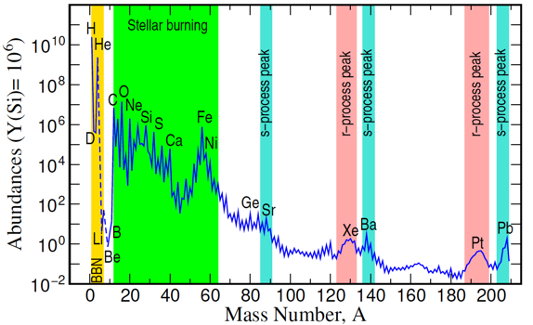
\includegraphics[scale=0.6]{solar_abunds}
\caption{
Abundances, Yi, of elements and their isotopes in the solar system as a function of mass number$\rm{A_i = Z_i + N_i}$ \cite{RevModPhys.93.015002}. The lightest particles were created in Big Bang, and the alpha particles were produced by stellar burning, and Type Ia supernovae make the iron peak. All the heavy elements are synthesized by s-process and r-process with three characteristic double peaks.
} 
\label{fig:solar_abunds}
\end{figure}
There are two processes involving the capture of free neutrons. The slow neutron capture process is much slower than $\beta$-decay reactions. Therefore, we refer to the s-process that primarily occurs within ordinary stars, particularly AGB stars, where the neutron flux is sufficient to cause neutron captures to recur every 10–100 years. The second is the rapid neutron capture process (r-process) which requires 100 captures per second, much higher than the $\beta$-decay rates. Since this process needs an extremely neutron-rich ($\rm{10^{23}}$ free neutrons per $\rm{cm^3}$)\cite{1957RvMP...29..547B} environment. Only core-collapse supernovae and binary neutron star mergers are supposed to be the production sites, more details in section 1.3. Except for these two processes, i, p, $\nu$, and $\nu p$ process can also create heavy elements. Since their contributions are minor, I will not introduce them here. Fig.\ref{fig:solar_abunds} shows the observed solar system abundances pattern as a function of A. Different colors indicate the production processes.  

\begin{figure}
\centering
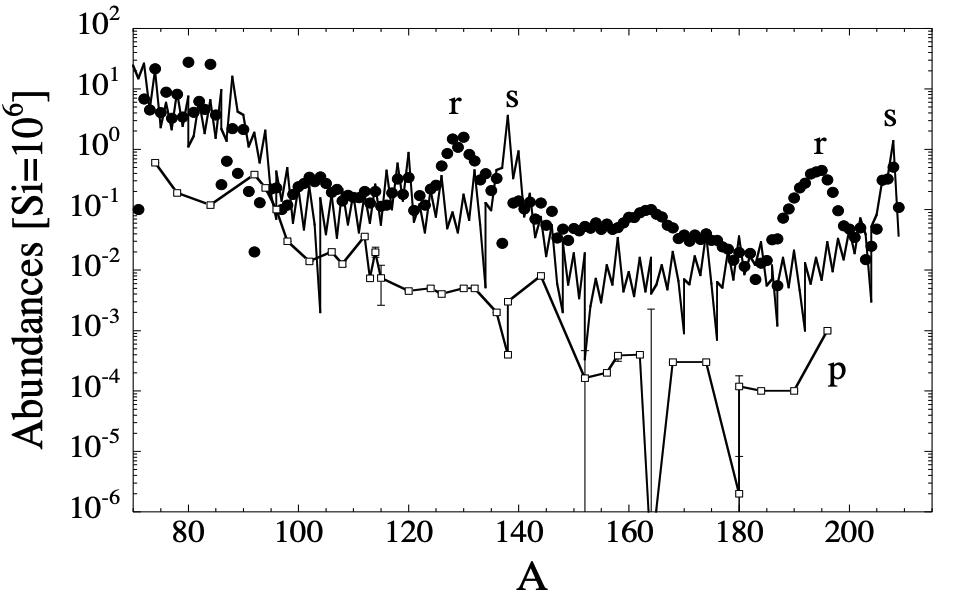
\includegraphics[scale=0.3]{decompose_solar}
\caption{
Decomposition of the solar abundances of heavy nuclides: s-process (solid line), r-process (dots), and p-process (squares).
}
\label{fig:decompose_solar}
\end{figure}

\subsection{1.2 R-process Abundances}
The theoretical r-process contribution is determined by subtracting theoretically predicted s-process and p-process yields from the measured solar abundances. When we investigate the r-process, we always compare our theoretical abundance pattern with the pattern shown in Fig.\ref{fig:decompose_solar}. The isotopic composition of the elements in our solar system is mostly based on the terrestrial data. The reason we choose this isotopic abundances pattern instead of the elemental abundances is that the terrestrial isotopic patterns are not affected to any significant level by geological processes.\cite{2007PhR...450...97A}. It's also easier to decompose s and r process isotopic elements. \cite{0004-637X-544-1-302} proved that the r-process abundances pattern is universal, which means the relative abundances observed in our solar system are the same in metal-poor (MP) halo stars. This also indicates that productions sites of those r-process elements are similar. Those MP halo stars were formed in the early stage of the Milky Way when the s-process did not have time to contaminate the abundances of the heavy elements. Therefore, those halo stars' data can provide us more information about how r-process elements were formed. Fig.\ref{fig:halo_samples} demonstrates the relative abundances of some r-process elements in five halo stars. Their abundances patterns are in agreement with each other.\\

The observed r-process isotopic abundance patterns show many distinct components. The first part is before the first peak with the mass number up to $\rm{A \sim 120}$. This region is believed to happen during the weak r-process in an environment where there are few neutron captures per seed (n/s $\sim$ 50)\cite{1996}, i.e., the neutrino-driven wind of core-collapse supernovae (CCSNe)\cite{1994ApJ...433..229W}. The second component is the main r-process, which happens in an environment with enough neutron captures per seed (n/s $\sim$ 100) to produce the two prominent peaks at A = 130 and 195 and a small peak around A = 165. Even though the two major peaks are generally considered due to closed neutron shells' long $\beta$ decay rates, the detailed formation process has not been explained yet. Besides, The formation process of the small peak around A = 160, known as rear earth peak (REP), has been explained by the funneling mechanism in 1997\cite{1997astro.ph..1007S} and 2012\cite{PhysRevC.85.045801}. However, more details about the flow of the abundance are still needed to understand this region fully. 

\begin{figure}
\centering
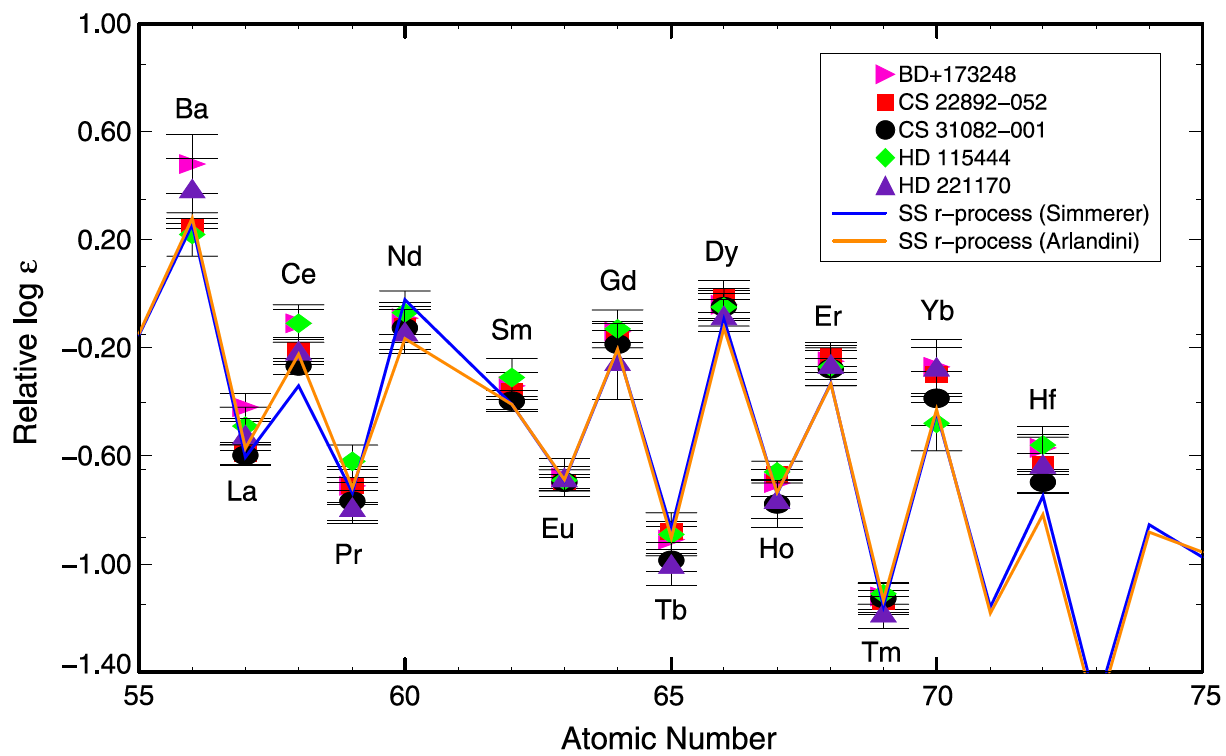
\includegraphics[scale=0.23]{halo_samples}
\caption{
Observed abundances of some heavy elements in five metal-poor halo stars. All stars have virtually identical relative abundances and that pattern also agrees with what is observed in the
our solar system (lines).
}
\label{fig:halo_samples}
\end{figure}

\subsection{1.3 Astrophysical Sites}\label{sec:astro}
Before we detail the whole r-process nucleosynthesis process, let us know more about the production sites since those sites provide the appropriate environment for the r-process, i.e., high temperature, high neutron to seed ratio. Super neutron-rich matter can be achieved by neutron stars. However, ejecting material from a deep gravitational neutron reservoir requires a cataclysmic event. So the possible sites are:
\begin{itemize}
\item 
The innermost ejecta of regular core-collapse supernovae. Specifically, the neutrino-driven wind and high entropy are responsible for the creation of r-process elements. 
\item Massive magneto-rotational supernovae (collapsars). Fast rotation and high magnetic fields are accountable for their explosion mechanism, producing neutron-rich jet ejecta along the poles or forming accretion disk outflows where the r-process nucleosynthesis happens.   
\item Ejecta from binary neutron star mergers or neutron
star black hole systems, which are naturally neutron-rich and have been considered extensively before the observation of GW170817. When two compact objects rotate around each other, once they emerge from spiral arms after the collision, matters there stay in a very neutron-rich environment and create robust r-process elements.
\end{itemize}
When matters are ejected from those events, they are firstly hot and dissociated. When temperature and density drop, they will experience many nuclear reactions, which will be discussed in the next section. 

\subsection{1.4 Evolving Stages in R-process Nucleosynthesis}
The nucleosynthesis of matter expanding from high temperature and density is well described as a descent of the hierarchy of statistical equilibria" \cite{1998PhRvC..58.3696M}. Each stage in the hierarchy is characterized by a set of rate-based constraints on the abundances which increase in number as time progresses in the expansion. For a system at constant temperature and volume, the change of free energy per neutron f is

\begin{equation}
df = \sum_{i} \mu_idY_i
\end{equation}

Where $\mu_i$ is the chemical potential, and $Y_i$ is the abundance per neutron of species i. Equilibrium abundances are those species that makes $df = 0$. Nuclear statistical equilibrium (NSE) reaches when there are minimum constraints: a fixed number of nucleons and a fixed electron-to-nucleon ratio $Y_e$. NSE means the reaction rate to combine free neutron and proton to nuclide (Z, A) is equal to the inverse rate. 
\begin{equation}
    (Z,A) \rightleftharpoons Z[p] + N[n]
\end{equation}

If the sum of abundances of some clusters C of species changes slowly until approximately fixed, those clusters are in quasi-equilibrium (QSE) condition. Inside each cluster, nuclides can exchange neutron and proton freely. However, the reaction between the two clusters is too slow to happen.  Once the sum of the abundance of every isotopic chine does not change, the isotopes in each chain are in $(n, \gamma)\rightleftharpoons (\gamma, n)$ equilibrium phase when the neutron capture rate and its inverse photo-disintegration rate are comparable. Still, the isotope chains are not in equilibrium with each other due to the slowness of charged-particle and $\beta^-$ decay rate that allow nuclei to flow from one element to another. The freeze-out from $(n, \gamma)\rightleftharpoons (\gamma, n)$ equilibrium and the decay back to stability are triggered by exhaustion of free neutrons. The abundances pattern formed in the freeze-out phase is what we observed in our solar system. 

\subsection{1.5 Freeze-out Phase}
The freeze-out phase is the last stage of r-process nucleosynthesis when nuclei slow their capture of neutrons and begin to decay back to stability. In this phase, the competition of nuclear reaction rates (neutron capture rate, photo-dissociation rate, and beta decay rate) is the key to forming the final abundances patterns. Both the final smooth abundance pattern and the REP are formed in this stage. Fig.\ref{fig:ng_final} shows the abundances distribution difference between the last time step of $(n, \gamma)\rightleftharpoons (\gamma, n)$ equilibrium and after the freeze-out phase. We can see the final smoothing abundances curve and the formation of REP.  Therefore, it is crucial to understand what happens in this final process.\\

\begin{figure}
\centering
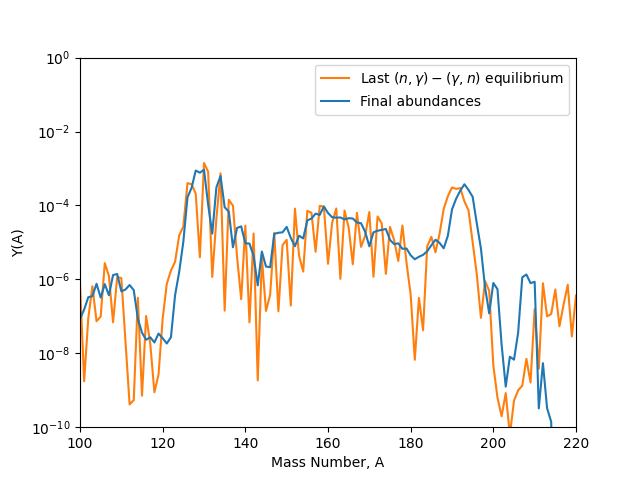
\includegraphics[scale=0.6]{ng_final}
\caption{
The abundances as a function of nucleon number for the last moment of $(n, \gamma)\rightleftharpoons (\gamma, n)$ equilibrium (orange) and the final abundances (blue).
}
\label{fig:ng_final}
\end{figure}

There are two scenarios during the final r-process in core-collapse supernovae. The first scenario is classical "hot" r process, which goes through an extended equilibrium between neutron captures and its inverse reaction at $T \sim 1$ GK until neutrons are exhausted. During this period, the beta-decay timescale (1/reaction rate) is longer than the other two $\tau_{(n,\gamma)} = \tau_{(\gamma, n)} \ll \tau_{\beta}$. The second scenario is "cold" r-process when the temperature drops below $\sim$ 0.5 GK, the photodissociation rate becomes slow. The following evolution proceeds by a competition between beta decay and neutron capture $\tau_{(n,\gamma)} \approx \tau_{\beta} \ll \tau_{(\gamma, n)}$\cite{PhysRevC.83.045809}. Those timescale evolution can be seen form Fig.\ref{fig:hot_cold}. The competition of those nuclear reactions forms the final r-process abundances pattern. 

\begin{figure}
\centering
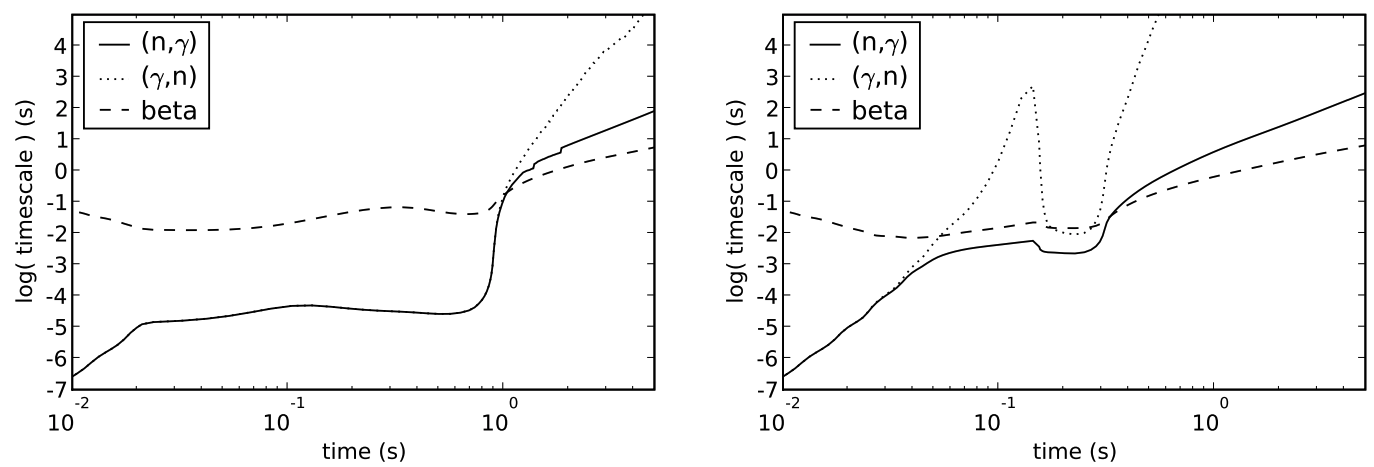
\includegraphics[scale=0.33]{hot_cold.png}
\caption{
Evolution of relevant timescales in classical "hot" r-process (left panel) and "cold" r-process (right panel). This is FIG. 3 in \cite{PhysRevC.83.045809}
}
\label{fig:hot_cold}
\end{figure}

\section{Research goals and method}
Within the two scenarios described above, the smooth abundances shape (or smoothing) is constructed. Besides, the two prominent r-process peaks, as well as the REP peak, are formed. What can this phenomenon tell us? From the nuclear physics part: what nuclear properties affect the final abundances pattern? Which element contributes more to the peaks before the final abundances shape form? From the astronomy part: Is the photo-dissociation reaction critical at the late time? Could this constrain the astrophysical conditions (i.e., the neutrino-driven wind)?  

\subsection{2.1 Research Goals}
With those questions in mind, my research goals are:
\begin{itemize}
    \item Understand how the smoothing happens
    \item Understand how the characteristic peaks are formed
    \item Understand the astronomical dynamic process at the late time of the r-process
\end{itemize}

\subsection{2.2 Research Steps}
\textbf{Steps for goal 1:} Fig.\ref{fig:ng_final} shows the abundances pattern at the last time step of $(n, \gamma)\rightleftharpoons (\gamma, n)$ equilibrium, which is also the starting time step of freeze-out. We now know that the spikes in the equilibrium abundance are due to the isotopic abundance peaks in each element. To know how the isotopic abundance curve spreads out, we need to look at the reactions after the equilibrium. When the equilibrium falls, both the neutron number density and the temperature decrease significantly. With the decrease of neutrons, the neutron capture rate will also drop dramatically. The competition between neutron capture, photo-dissociation, and $\beta$ decay rate is what we will focus on.\\

Branching theory is a kind of "language" that can describe the species' abundance flow path. It can also give us the relative contribution from one species to another species. With this method and the correct reaction rates, we can understand how the nuclides' abundances evolve with time and why they behave as they do. I will start from a simple case with only two isotopic chains with and without the photo-dissociation rate corresponding to "cold" and "hot" freeze-out phase. Once we understand the simple model, we can add more isotopic chains to get the final r-process abundance pattern after the freeze-out phase.\\

\textbf{Steps for goal 2:} 
When we understand the smoothing process, we can also use branching theory to look into the detail in the REP (A $\sim$ 165). The funneling mechanism in explaining the formation of REP is a general method. As for how the nuclides react to each other and which path the nuclides take to form the peak in the local REP region are still unclear. We will also start from two isotopic chains in "cold" and "hot" cases looking at the surrounding nuclides' contribution to the specific nuclide. Once we know the most popular path the isotopes choose, we will enlarge our local REP area to include more isotopic chains. The details of the flow of the abundance will explain how the nuclides flow to the REP.\\

\textbf{Steps for goal 3:} 
Since the REP forms only at the late r-process, the astrophysical condition is a crucial factor affecting the final abundances distribution. We will put different astrophysical conditions to our r-process network calculation. And then compare the simulated abundances pattern with the observed solar r-process abundance pattern to find the best astrophysical sites. If we can pinpoint the local region and the environment requirements for the formation of the REP, we can narrower the astrophysical conditions for the r-process nucleosynthesis site: hot, cold, or very neutron-rich cold...\\
\clearpage

\bibliography{clemson}
\end{document}
